\documentclass[crop]{standalone}

\usepackage[dvipsnames]{xcolor}
\usepackage{tikz}

\usetikzlibrary{backgrounds}

\begin{document}
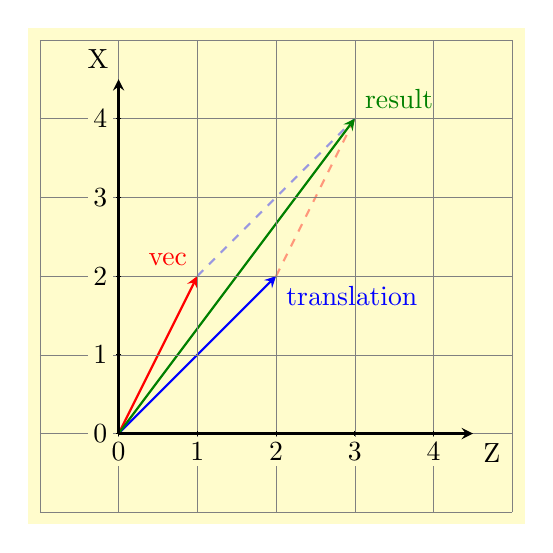
\begin{tikzpicture}[background rectangle/.style={fill=yellow!20}, show background rectangle]

	\draw[thick,-stealth,red] (0,0) -- (1,2) node[anchor=south east] {vec};
	\draw[thick,-stealth,blue] (0,0) -- (2,2) node[anchor=north west] {translation};
	\draw[thick,blue,dashed,opacity=0.4] (1,2) -- (3,4);
	\draw[thick,red,dashed,opacity=0.4] (2,2) -- (3,4);
	\draw[thick,-stealth,Green] (0,0) -- (3,4) node[anchor=south west] {result};


	\draw[step=1cm,gray,very thin] (-1,-1) grid (5,5);
	\draw[thick,-stealth] (0,0) -- (4.5,0) node[anchor=north west] {Z};
	\draw[thick,-stealth] (0,0) -- (0,4.5) node[anchor=south east] {X};
	\foreach \z in {0,1,2,3,4}
		\draw (\z cm,1pt) -- (\z cm,-1pt) node[anchor=north, inner sep=2pt, outer xsep=1.1pt, fill=yellow!20] {$\z$};
	\foreach \x in {0,1,2,3,4}
		\draw (1pt,\x cm) -- (-1pt,\x cm) node[anchor=east, inner sep=2pt, outer xsep=1.1pt, fill=yellow!20] {$\x$};

\end{tikzpicture}
\end{document}


% \begin{document}
% \begin{tikzpicture}[background rectangle/.style={fill=yellow!20}, show background rectangle]

% 	\draw[thick,-stealth,red] (0,0) -- (-1,2) node[anchor=south west] {vec};
% 	\draw[thick,-stealth,blue] (0,0) -- (-2,2) node[anchor=north east] {translation};
% 	\draw[thick,blue,dashed,opacity=0.4] (-1,2) -- (-3,4);
% 	\draw[thick,red,dashed,opacity=0.4] (-2,2) -- (-3,4);
% 	\draw[thick,-stealth,Green] (0,0) -- (-3,4) node[anchor=south east] {result};


% 	\draw[step=1cm,gray,very thin] (-5,-1) grid (1,5);
% 	\draw[thick,-stealth] (0,0) -- (-4.5,0) node[anchor=north east] {X};
% 	\draw[thick,-stealth] (0,0) -- (0,4.5) node[anchor=south west] {Z};
% 	\foreach \z in {0,1,2,3,4}
% 		\draw (1pt,\z cm) -- (-1pt,\z cm) node[anchor=west, inner sep=1.5pt, outer xsep=4pt, fill=yellow!20] {$\z$};
% 	\foreach \x in {0,1,2,3,4}
% 		\draw (-\x cm,1pt) -- (-\x cm,-1pt) node[anchor=north, inner sep=1.5pt, outer ysep=2pt, fill=yellow!20] {$\x$};

% \end{tikzpicture}
% \end{document}
